\documentclass{article}
\usepackage[preprint]{neurips_2024}
\usepackage[utf8]{inputenc}
\usepackage[T1]{fontenc}
\usepackage[colorlinks=true,linkcolor=black,citecolor=blue!50!black,urlcolor=blue!50!black]{hyperref}
\usepackage{url}
\usepackage{booktabs}
\usepackage{amsmath,amssymb,amsthm}
\usepackage{cancel}
\usepackage{microtype}
\usepackage{xcolor}
\usepackage{tikz}
\usetikzlibrary{arrows.meta,positioning}

\newtheorem{proposition}{Proposition}[section]
\newtheorem{lemma}[proposition]{Lemma}
\newtheorem{corollary}[proposition]{Corollary}
\theoremstyle{definition}
\newtheorem{definition}[proposition]{Definition}
\newtheorem{assumption}{Assumption}
\theoremstyle{remark}
\newtheorem{remark}[proposition]{Remark}

\newcommand{\E}{\mathbb{E}}
\newcommand{\dE}{\Delta E}
\newcommand{\dP}{\Delta P}
\newcommand{\Ob}{\bar O}
\newcommand{\KL}{\mathrm{KL}}
\newcommand{\why}[1]{\tag*{\small(#1)}}

\title{The State Defect, Empowerment and Plasticity}

\author{XXX}

\begin{document}
\maketitle

\begin{abstract}
For an agent that acts on a memory, we derive the empowerment and plasticity mismatches between the history and the memory, the two splits of the state defect, and three ways to separate the reward inside them. We then compare the Bellman equation with the history as the state and the same equation with the memory as the state. They differ only in the prediction of the next observation, and these two predictions are the ones the state defect compares. Subtracting the two equations step by step writes the gap between the two values, for a finite and for the infinite horizon, as a discounted sum of comparisons of the predictions of the agent's one-step defects $D_t,D_{t+1},D_{t+2},\dots$, and these defects bound it. Every derivation is written term by term, and every cancellation names the assumption or lemma that allows it.
\end{abstract}

\section{Setting}\label{sec:setting}

\begin{center}
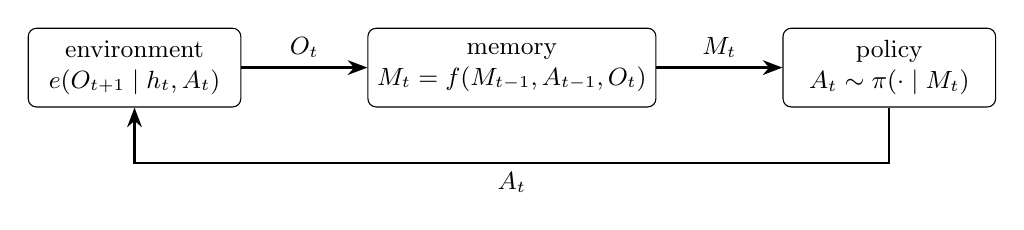
\begin{tikzpicture}[>={Stealth[length=2.5mm]}, node distance=10mm and 16mm,
  box/.style={draw, rounded corners=3pt, minimum height=10mm, minimum width=27mm, align=center, font=\small}]
\node[box] (world) {environment\\ $e(O_{t+1}\mid h_t, A_t)$};
\node[box, right=of world] (mem) {memory\\ $M_t = f(M_{t-1}, A_{t-1}, O_t)$};
\node[box, right=of mem] (pol) {policy\\ $A_t \sim \pi(\cdot \mid M_t)$};
\draw[->, thick] (world) -- node[above, font=\small] {$O_t$} (mem);
\draw[->, thick] (mem) -- node[above, font=\small] {$M_t$} (pol);
\draw[->, thick] (pol.south) -- ++(0,-7mm) -| node[pos=0.25, below, font=\small] {$A_t$} (world.south);
\end{tikzpicture}
\end{center}

The history is $h_t=(O_1,A_1,\dots,A_{t-1},O_t)$. The observation contains the reward: $O_t=(R_t,\Ob_t)$, with $\Ob_t$ the rest of the observation. All observation and action sets are finite, and all probabilities are under the law of the agent's experience induced by the three boxes.

\begin{assumption}[Environment]\label{as:env}
$O_{t+1}\sim e(\cdot\mid h_t,A_t)$ for some law $e$; the environment may depend on the whole history, with no Markov or stationarity condition.
\end{assumption}

\begin{assumption}[Memory]\label{as:mem}
$M_1=f_1(O_1)$ and $M_{t+1}=f(M_t,A_t,O_{t+1})$ for fixed maps $f_1,f$. Hence $M_t$ is a function of $h_t$.
\end{assumption}

\begin{assumption}[Policy]\label{as:pol}
$P(A_t=a\mid h_t)=\pi(a\mid M_t)$: the action depends on the history only through the memory.
\end{assumption}

Every identity in this note was checked numerically. The script \texttt{checks/verify\_note.py} computes the exact law of all trajectories in small random environments whose next observation depends on the whole history, and tests each numbered statement for a finite horizon; the largest error is $10^{-13}$. The infinite-horizon statements are limits of the finite ones.

\section{Tools}\label{sec:tools}

We use five standard facts \citep[Ch.~2]{cover2006elements}. $X,Y,W,Z$ are random variables, and conditioning on nothing is allowed.
\begin{enumerate}
\item[(T1)] $I(X;Y\mid Z)=H(X\mid Z)-H(X\mid Y,Z)=H(Y\mid Z)-H(Y\mid X,Z)$.
\item[(T2)] Chain rule: $I(X,Y;W\mid Z)=I(X;W\mid Z)+I(Y;W\mid Z,X)=I(Y;W\mid Z)+I(X;W\mid Z,Y)$, and the same with the pair in the second place, since $I$ is symmetric.
\item[(T3)] $I(X;Y\mid Z)\ge0$, with equality exactly when $X$ and $Y$ are independent given $Z$.
\item[(T4)] If $W$ is a function of $X$, conditioning on $(X,W)$ is the same as conditioning on $X$: $H(Y\mid X,W,Z)=H(Y\mid X,Z)$. By Assumption~\ref{as:mem}, this applies to $W=M_t$, $X=h_t$.
\item[(T5)] $h_{t+1}=(h_t,A_t,O_{t+1})$, so conditioning on $h_{t+1}$ is the same as conditioning on $(h_t,A_t,O_{t+1})$.
\end{enumerate}

\begin{lemma}[The action depends on the past only through the memory]\label{lem:action}
Under Assumptions~\ref{as:mem} and~\ref{as:pol}, for every $k\ge0$,
\[
H(A_{t+k}\mid h_t,A_t,O_{t+1},\dots,A_{t+k-1},O_{t+k})=H(A_{t+k}\mid M_t,A_t,O_{t+1},\dots,A_{t+k-1},O_{t+k}),
\]
and therefore $I(h_t;A_{t+k}\mid M_t,A_t,O_{t+1},\dots,A_{t+k-1},O_{t+k})=0$. The cases used most are
\begin{align*}
\text{(a) } k=0:&\quad H(A_t\mid h_t)=H(A_t\mid M_t),\\
\text{(b) } k=1:&\quad H(A_{t+1}\mid h_t,A_t,O_{t+1})=H(A_{t+1}\mid M_t,A_t,O_{t+1}).
\end{align*}
\end{lemma}

\begin{proof}
By (T5) applied $k$ times, the conditioning variables on the left are $h_{t+k}$. By Assumption~\ref{as:pol}, the law of $A_{t+k}$ given $h_{t+k}$ is $\pi(\cdot\mid M_{t+k})$. By Assumption~\ref{as:mem}, $M_{t+k}$ is obtained from $M_t$ by applying $f$ $k$ times with the inputs $(A_t,O_{t+1}),\dots,(A_{t+k-1},O_{t+k})$, so it is a function of the conditioning variables on the right. These variables are a function of $h_{t+k}$, so the law of $A_{t+k}$ given them is the average of $\pi(\cdot\mid M_{t+k})$ over the histories consistent with them, which is $\pi(\cdot\mid M_{t+k})$ itself. Both laws are $\pi(\cdot\mid M_{t+k})$, so the two entropies are equal. For the mutual information, write $C=(A_t,O_{t+1},\dots,A_{t+k-1},O_{t+k})$ in this proof only:
\begin{align*}
I(h_t;A_{t+k}\mid M_t,C)
&=H(A_{t+k}\mid M_t,C)-H(A_{t+k}\mid h_t,M_t,C) \why{T1}\\
&=H(A_{t+k}\mid M_t,C)-H(A_{t+k}\mid h_t,C) \why{T4}\\
&=0 \why{the equality of entropies above}.
\end{align*}
\end{proof}
\section{Empowerment and plasticity at the history and at the memory}\label{sec:EP}

In every derivation below, the label at the right of a line names the fact used to obtain that line. Two struck-through terms in a line are equal by the named fact and cancel.

\begin{definition}\label{def:EP}
Following the one-step form of \citet{abel2025plasticity}, the empowerment of the action and the plasticity of the next action, computed from the history and from the memory, are
\begin{align*}
E_t&=I(A_t;O_{t+1}\mid h_t), & E_t(M)&=I(A_t;O_{t+1}\mid M_t),\\
P_{t+1}&=I(O_{t+1};A_{t+1}\mid h_t,A_t), & P_{t+1}(M)&=I(O_{t+1};A_{t+1}\mid M_t,A_t),
\end{align*}
and the two mismatches are $\dE_t=E_t-E_t(M)$ and $\dP_t=P_{t+1}(M)-P_{t+1}$.
\end{definition}

\begin{proposition}[Empowerment mismatch]\label{prop:dE}
Under Assumptions~\ref{as:mem} and~\ref{as:pol}, $\dE_t=I(h_t;A_t\mid M_t,O_{t+1})\ge0$.
\end{proposition}

\begin{proof}
Write both empowerments with (T1), with $A_t$ as the variable whose entropy is taken:
\begin{align*}
E_t&=H(A_t\mid h_t)-H(A_t\mid h_t,O_{t+1}),\\
E_t(M)&=H(A_t\mid M_t)-H(A_t\mid M_t,O_{t+1}).
\end{align*}
Subtract:
\begin{align*}
\dE_t&=\cancel{H(A_t\mid h_t)}-H(A_t\mid h_t,O_{t+1})-\cancel{H(A_t\mid M_t)}+H(A_t\mid M_t,O_{t+1}) \why{struck terms equal, Lemma~\ref{lem:action}(a)}\\
&=H(A_t\mid M_t,O_{t+1})-H(A_t\mid h_t,O_{t+1})\\
&=H(A_t\mid M_t,O_{t+1})-H(A_t\mid h_t,M_t,O_{t+1}) \why{T4}\\
&=I(h_t;A_t\mid M_t,O_{t+1}) \why{T1},
\end{align*}
which is nonnegative by (T3).
\end{proof}

\begin{proposition}[Plasticity mismatch]\label{prop:dP}
Under Assumptions~\ref{as:mem} and~\ref{as:pol}, $\dP_t=I(h_t;A_{t+1}\mid M_t,A_t)\ge0$.
\end{proposition}

\begin{proof}
Write both plasticities with (T1), with $A_{t+1}$ as the variable whose entropy is taken:
\begin{align*}
P_{t+1}&=H(A_{t+1}\mid h_t,A_t)-H(A_{t+1}\mid h_t,A_t,O_{t+1}),\\
P_{t+1}(M)&=H(A_{t+1}\mid M_t,A_t)-H(A_{t+1}\mid M_t,A_t,O_{t+1}).
\end{align*}
Subtract:
\begin{align*}
\dP_t&=H(A_{t+1}\mid M_t,A_t)-\cancel{H(A_{t+1}\mid M_t,A_t,O_{t+1})}\\
&\quad-H(A_{t+1}\mid h_t,A_t)+\cancel{H(A_{t+1}\mid h_t,A_t,O_{t+1})} \why{struck terms equal, Lemma~\ref{lem:action}(b)}\\
&=H(A_{t+1}\mid M_t,A_t)-H(A_{t+1}\mid h_t,A_t)\\
&=H(A_{t+1}\mid M_t,A_t)-H(A_{t+1}\mid h_t,M_t,A_t) \why{T4}\\
&=I(h_t;A_{t+1}\mid M_t,A_t) \why{T1},
\end{align*}
which is nonnegative by (T3).
\end{proof}

In words: given the outcome, the history still tells something about the action that the memory does not, so the memory underestimates empowerment; and the history tells something about the next action that the memory does not, so the memory overestimates plasticity.

\section{The state defect and its two splits}\label{sec:splits}

\begin{definition}\label{def:terms}
The state defect and two further terms are
\[
D_t=I(h_t;O_{t+1}\mid M_t,A_t),\qquad D^0_t=I(h_t;O_{t+1}\mid M_t),\qquad D^+_t=I(h_t;O_{t+1}\mid M_t,A_t,A_{t+1}).
\]
With Propositions~\ref{prop:dE} and~\ref{prop:dP}, each of the five terms is a mutual information between the history and one variable, given the memory and other variables:
\begin{center}
\small
\begin{tabular}{llll}
\toprule
term & mutual information & variable predicted & given, besides $M_t$\\
\midrule
$D_t$ & $I(h_t;O_{t+1}\mid M_t,A_t)$ & $O_{t+1}$ & $A_t$\\
$D^0_t$ & $I(h_t;O_{t+1}\mid M_t)$ & $O_{t+1}$ & nothing\\
$\dE_t$ & $I(h_t;A_t\mid M_t,O_{t+1})$ & $A_t$ & $O_{t+1}$\\
$\dP_t$ & $I(h_t;A_{t+1}\mid M_t,A_t)$ & $A_{t+1}$ & $A_t$\\
$D^+_t$ & $I(h_t;O_{t+1}\mid M_t,A_t,A_{t+1})$ & $O_{t+1}$ & $A_t,A_{t+1}$\\
\bottomrule
\end{tabular}
\end{center}
By (T1) and (T4), each is the uncertainty about the predicted variable given the memory minus the uncertainty given the history.
\end{definition}

\begin{proposition}[First split]\label{prop:split1}
Under Assumptions~\ref{as:mem} and~\ref{as:pol}, $D_t=D^0_t+\dE_t$.
\end{proposition}

\begin{proof}
Apply (T2) to $I(h_t,A_t;O_{t+1}\mid M_t)$ in the two orders.

History first:
\begin{align*}
I(h_t,A_t;O_{t+1}\mid M_t)&=I(h_t;O_{t+1}\mid M_t)+I(A_t;O_{t+1}\mid M_t,h_t) \why{T2}\\
&=D^0_t+I(A_t;O_{t+1}\mid h_t) \why{Definition~\ref{def:terms}; T4}\\
&=D^0_t+E_t \why{Definition~\ref{def:EP}}.
\end{align*}
Action first:
\begin{align*}
I(h_t,A_t;O_{t+1}\mid M_t)&=I(A_t;O_{t+1}\mid M_t)+I(h_t;O_{t+1}\mid M_t,A_t) \why{T2}\\
&=E_t(M)+D_t \why{Definitions~\ref{def:EP} and~\ref{def:terms}}.
\end{align*}
The two right sides are equal, so $D^0_t+E_t=E_t(M)+D_t$, that is, $D_t=D^0_t+E_t-E_t(M)=D^0_t+\dE_t$.
\end{proof}

\begin{proposition}[Second split]\label{prop:split2}
Under Assumptions~\ref{as:mem} and~\ref{as:pol}, $D_t=\dP_t+D^+_t$.
\end{proposition}

\begin{proof}
Apply (T2) to $I(h_t;O_{t+1},A_{t+1}\mid M_t,A_t)$ in the two orders.

Next observation first:
\begin{align*}
I(h_t;O_{t+1},A_{t+1}\mid M_t,A_t)&=I(h_t;O_{t+1}\mid M_t,A_t)+I(h_t;A_{t+1}\mid M_t,A_t,O_{t+1}) \why{T2}\\
&=D_t+0 \why{Definition~\ref{def:terms}; Lemma~\ref{lem:action}, $k=1$}.
\end{align*}
Next action first:
\begin{align*}
I(h_t;O_{t+1},A_{t+1}\mid M_t,A_t)&=I(h_t;A_{t+1}\mid M_t,A_t)+I(h_t;O_{t+1}\mid M_t,A_t,A_{t+1}) \why{T2}\\
&=\dP_t+D^+_t \why{Proposition~\ref{prop:dP}; Definition~\ref{def:terms}}.
\end{align*}
The two right sides are equal.
\end{proof}

\begin{remark}[Both splits come from one quantity]\label{rem:orders}
Apply (T2) to $I(h_t;A_t,O_{t+1},A_{t+1}\mid M_t)$ in three orders. In the order of time, $(A_t,O_{t+1},A_{t+1})$, the terms are $I(h_t;A_t\mid M_t)=0$ (Lemma~\ref{lem:action}, $k=0$), $D_t$, and $I(h_t;A_{t+1}\mid M_t,A_t,O_{t+1})=0$ (Lemma~\ref{lem:action}, $k=1$). In the order $(O_{t+1},A_t,A_{t+1})$ they are $D^0_t$, $\dE_t$ and $I(h_t;A_{t+1}\mid M_t,O_{t+1},A_t)=0$. In the order $(A_t,A_{t+1},O_{t+1})$ they are $0$, $\dP_t$ and $D^+_t$. So the first split reads the action $A_t$ after the observation it produced, the second reads the next action $A_{t+1}$ before the observation it responds to, and in the order of time the two actions contribute nothing.
\end{remark}

\begin{corollary}\label{cor:consequences}
Under Assumptions~\ref{as:mem} and~\ref{as:pol}:
\begin{enumerate}
\item[(a)] $D_t=0$ if and only if $D^0_t=0$ and $\dE_t=0$, and if and only if $\dP_t=0$ and $D^+_t=0$;
\item[(b)] $\dP_t\le D_t$;
\item[(c)] $\dE_t\le H(A_t\mid M_t)$, so $\dE_t=0$ and $D_t=D^0_t$ when the policy is deterministic.
\end{enumerate}
\end{corollary}

\begin{proof}
(a) Each term is nonnegative (T3), and a sum of two nonnegative terms is zero exactly when both are. (b) From Proposition~\ref{prop:split2}, since $D^+_t\ge0$. (c) $\dE_t=H(A_t\mid M_t,O_{t+1})-H(A_t\mid h_t,O_{t+1})\le H(A_t\mid M_t,O_{t+1})\le H(A_t\mid M_t)$, where the first step drops a nonnegative entropy and the second uses that conditioning does not increase entropy, which is (T1) with (T3). A deterministic policy has $H(A_t\mid M_t)=0$; then Proposition~\ref{prop:split1} gives $D_t=D^0_t$.
\end{proof}

\section{Separating the reward}\label{sec:reward}

The observation is a pair, $O_{t+1}=(R_{t+1},\Ob_{t+1})$. We first split each term by a general pair $O_{t+1}=(X,Y)$, with $X$ taken first, and then consider three ways to separate the reward: reward first, $(X,Y)=(R_{t+1},\Ob_{t+1})$; rest first, $(X,Y)=(\Ob_{t+1},R_{t+1})$; and a partial information decomposition, which takes no order.

\subsection{A split by $O_{t+1}=(X,Y)$}

\begin{proposition}[$D_t$, $D^0_t$ and $D^+_t$]\label{prop:xy-D}
For $O_{t+1}=(X,Y)$,
\begin{align*}
D_t&=I(h_t;X\mid M_t,A_t)+I(h_t;Y\mid M_t,A_t,X),\\
D^0_t&=I(h_t;X\mid M_t)+I(h_t;Y\mid M_t,X),\\
D^+_t&=I(h_t;X\mid M_t,A_t,A_{t+1})+I(h_t;Y\mid M_t,A_t,A_{t+1},X),
\end{align*}
and every term on the right is nonnegative.
\end{proposition}

\begin{proof}
Each line is (T2) applied to $I(h_t;X,Y\mid\cdot)$ with $X$ first, and each term is nonnegative by (T3).
\end{proof}

\begin{proposition}[$\dE_t$]\label{prop:xy-E}
Under Assumptions~\ref{as:mem} and~\ref{as:pol}, for $O_{t+1}=(X,Y)$,
\[
\dE_t=\underbrace{\big[I(A_t;X\mid h_t)-I(A_t;X\mid M_t)\big]}_{X\text{ part}}+\underbrace{\big[I(A_t;Y\mid h_t,X)-I(A_t;Y\mid M_t,X)\big]}_{Y\text{ part}},
\]
where the $X$ part equals $I(h_t;A_t\mid M_t,X)\ge0$ and the $Y$ part can be negative.
\end{proposition}

\begin{proof}
By (T2), with $X$ first,
\begin{align*}
E_t&=I(A_t;X,Y\mid h_t)=I(A_t;X\mid h_t)+I(A_t;Y\mid h_t,X),\\
E_t(M)&=I(A_t;X,Y\mid M_t)=I(A_t;X\mid M_t)+I(A_t;Y\mid M_t,X).
\end{align*}
Subtracting and grouping the $X$ terms and the $Y$ terms gives the formula for $\dE_t=E_t-E_t(M)$. For the $X$ part, write both terms with (T1), with $A_t$ as the variable whose entropy is taken:
\begin{align*}
&I(A_t;X\mid h_t)-I(A_t;X\mid M_t)\\
&\quad=\cancel{H(A_t\mid h_t)}-H(A_t\mid h_t,X)-\cancel{H(A_t\mid M_t)}+H(A_t\mid M_t,X) \why{struck terms equal, Lemma~\ref{lem:action}(a)}\\
&\quad=H(A_t\mid M_t,X)-H(A_t\mid h_t,M_t,X) \why{T4}\\
&\quad=I(h_t;A_t\mid M_t,X) \why{T1}.
\end{align*}
The $Y$ part is a difference of two mutual informations with different conditioning, and no lemma relates them.
\end{proof}

\begin{proposition}[$\dP_t$]\label{prop:xy-P}
Under Assumptions~\ref{as:mem} and~\ref{as:pol}, for $O_{t+1}=(X,Y)$,
\[
\begin{aligned}
\dP_t&=\underbrace{\big[I(X;A_{t+1}\mid M_t,A_t)-I(X;A_{t+1}\mid h_t,A_t)\big]}_{X\text{ part}}\\
&\quad+\underbrace{\big[I(Y;A_{t+1}\mid M_t,A_t,X)-I(Y;A_{t+1}\mid h_t,A_t,X)\big]}_{Y\text{ part}},
\end{aligned}
\]
where the $Y$ part equals $I(h_t;A_{t+1}\mid M_t,A_t,X)\ge0$ and the $X$ part can be negative.
\end{proposition}

\begin{proof}
By (T2), with $X$ first,
\begin{align*}
P_{t+1}&=I(X,Y;A_{t+1}\mid h_t,A_t)=I(X;A_{t+1}\mid h_t,A_t)+I(Y;A_{t+1}\mid h_t,A_t,X),\\
P_{t+1}(M)&=I(X,Y;A_{t+1}\mid M_t,A_t)=I(X;A_{t+1}\mid M_t,A_t)+I(Y;A_{t+1}\mid M_t,A_t,X).
\end{align*}
Subtracting gives the formula for $\dP_t=P_{t+1}(M)-P_{t+1}$. For the $Y$ part, write both terms with (T1), with $A_{t+1}$ as the variable whose entropy is taken, and use $(X,Y)=O_{t+1}$:
\begin{align*}
&I(Y;A_{t+1}\mid M_t,A_t,X)-I(Y;A_{t+1}\mid h_t,A_t,X)\\
&\quad=H(A_{t+1}\mid M_t,A_t,X)-\cancel{H(A_{t+1}\mid M_t,A_t,O_{t+1})}\\
&\qquad-H(A_{t+1}\mid h_t,A_t,X)+\cancel{H(A_{t+1}\mid h_t,A_t,O_{t+1})} \why{struck terms equal, Lemma~\ref{lem:action}(b)}\\
&\quad=H(A_{t+1}\mid M_t,A_t,X)-H(A_{t+1}\mid h_t,M_t,A_t,X) \why{T4}\\
&\quad=I(h_t;A_{t+1}\mid M_t,A_t,X) \why{T1}.
\end{align*}
The $X$ part is a difference of two mutual informations with different conditioning, and no lemma relates them.
\end{proof}

\begin{proposition}[The two splits for each part]\label{prop:xy-splits}
Under Assumptions~\ref{as:mem} and~\ref{as:pol}, for $O_{t+1}=(X,Y)$, the $X$ part and the $Y$ part of $D_t$ each split in the two ways of Section~\ref{sec:splits}:
\begin{align*}
I(h_t;X\mid M_t,A_t)&=I(h_t;X\mid M_t)+\big[I(A_t;X\mid h_t)-I(A_t;X\mid M_t)\big] \tag*{\small first split}\\
&=\big[I(X;A_{t+1}\mid M_t,A_t)-I(X;A_{t+1}\mid h_t,A_t)\big]+I(h_t;X\mid M_t,A_t,A_{t+1}) \tag*{\small second split},\\[4pt]
I(h_t;Y\mid M_t,A_t,X)&=I(h_t;Y\mid M_t,X)+\big[I(A_t;Y\mid h_t,X)-I(A_t;Y\mid M_t,X)\big] \tag*{\small first split}\\
&=I(h_t;A_{t+1}\mid M_t,A_t,X)+I(h_t;Y\mid M_t,A_t,A_{t+1},X) \tag*{\small second split}.
\end{align*}
So each part of $D_t$ is the sum of the same part of $D^0_t$ and of $\dE_t$, and of the same part of $\dP_t$ and of $D^+_t$.
\end{proposition}

\begin{proof}
\emph{$X$ part, first split.} Apply (T2) to $I(h_t,A_t;X\mid M_t)$ in two orders:
\begin{align*}
I(h_t,A_t;X\mid M_t)&=I(h_t;X\mid M_t)+I(A_t;X\mid M_t,h_t)=I(h_t;X\mid M_t)+I(A_t;X\mid h_t) \why{T2; T4}\\
&=I(A_t;X\mid M_t)+I(h_t;X\mid M_t,A_t) \why{T2}.
\end{align*}
Equate the two lines and solve for $I(h_t;X\mid M_t,A_t)$.

\emph{$X$ part, second split.} Write the $X$ part of $\dP_t$ with (T1), with $X$ as the variable whose entropy is taken, and regroup:
\begin{align*}
&I(X;A_{t+1}\mid M_t,A_t)-I(X;A_{t+1}\mid h_t,A_t)\\
&\quad=\big[H(X\mid M_t,A_t)-H(X\mid M_t,A_t,A_{t+1})\big]-\big[H(X\mid h_t,A_t)-H(X\mid h_t,A_t,A_{t+1})\big] \why{T1}\\
&\quad=\big[H(X\mid M_t,A_t)-H(X\mid h_t,A_t)\big]-\big[H(X\mid M_t,A_t,A_{t+1})-H(X\mid h_t,A_t,A_{t+1})\big] \why{regroup}\\
&\quad=I(h_t;X\mid M_t,A_t)-I(h_t;X\mid M_t,A_t,A_{t+1}) \why{T4; T1}.
\end{align*}
Move the last term to the left side.

\emph{$Y$ part, first split.} Apply (T2) to $I(h_t,A_t;Y\mid M_t,X)$ in two orders:
\begin{align*}
I(h_t,A_t;Y\mid M_t,X)&=I(h_t;Y\mid M_t,X)+I(A_t;Y\mid h_t,X) \why{T2; T4}\\
&=I(A_t;Y\mid M_t,X)+I(h_t;Y\mid M_t,A_t,X) \why{T2}.
\end{align*}
Equate and solve for $I(h_t;Y\mid M_t,A_t,X)$.

\emph{$Y$ part, second split.} Apply (T2) to $I(h_t;Y,A_{t+1}\mid M_t,A_t,X)$ in two orders:
\begin{align*}
I(h_t;Y,A_{t+1}\mid M_t,A_t,X)&=I(h_t;Y\mid M_t,A_t,X)+I(h_t;A_{t+1}\mid M_t,A_t,X,Y) \why{T2}\\
&=I(h_t;Y\mid M_t,A_t,X)+0 \why{$(X,Y)=O_{t+1}$; Lemma~\ref{lem:action}, $k=1$}\\
I(h_t;Y,A_{t+1}\mid M_t,A_t,X)&=I(h_t;A_{t+1}\mid M_t,A_t,X)+I(h_t;Y\mid M_t,A_t,A_{t+1},X) \why{T2}.
\end{align*}
Equate the two.
\end{proof}

So, whichever part comes first, its empowerment part is nonnegative and its plasticity part is signed; for the part that comes second, it is the other way round.

\subsection{Reward first and rest first}

Propositions~\ref{prop:xy-D}--\ref{prop:xy-P} with the two choices of $(X,Y)$ give the following. In every line, the term on the left is the sum of its reward part and its rest part. Every term written as a single mutual information is nonnegative; the terms in brackets can be negative.

\paragraph{Reward first,} $(X,Y)=(R_{t+1},\Ob_{t+1})$: the reward part comes first in each line.
\begin{align*}
D_t&=I(h_t;R_{t+1}\mid M_t,A_t)+I(h_t;\Ob_{t+1}\mid M_t,A_t,R_{t+1}),\\
D^0_t&=I(h_t;R_{t+1}\mid M_t)+I(h_t;\Ob_{t+1}\mid M_t,R_{t+1}),\\
D^+_t&=I(h_t;R_{t+1}\mid M_t,A_t,A_{t+1})+I(h_t;\Ob_{t+1}\mid M_t,A_t,A_{t+1},R_{t+1}),\\
\dE_t&=I(h_t;A_t\mid M_t,R_{t+1})+\big[I(A_t;\Ob_{t+1}\mid h_t,R_{t+1})-I(A_t;\Ob_{t+1}\mid M_t,R_{t+1})\big],\\
\dP_t&=\big[I(R_{t+1};A_{t+1}\mid M_t,A_t)-I(R_{t+1};A_{t+1}\mid h_t,A_t)\big]+I(h_t;A_{t+1}\mid M_t,A_t,R_{t+1}).
\end{align*}

\paragraph{Rest first,} $(X,Y)=(\Ob_{t+1},R_{t+1})$: the reward part comes second in each line.
\begin{align*}
D_t&=I(h_t;\Ob_{t+1}\mid M_t,A_t)+I(h_t;R_{t+1}\mid M_t,A_t,\Ob_{t+1}),\\
D^0_t&=I(h_t;\Ob_{t+1}\mid M_t)+I(h_t;R_{t+1}\mid M_t,\Ob_{t+1}),\\
D^+_t&=I(h_t;\Ob_{t+1}\mid M_t,A_t,A_{t+1})+I(h_t;R_{t+1}\mid M_t,A_t,A_{t+1},\Ob_{t+1}),\\
\dE_t&=I(h_t;A_t\mid M_t,\Ob_{t+1})+\big[I(A_t;R_{t+1}\mid h_t,\Ob_{t+1})-I(A_t;R_{t+1}\mid M_t,\Ob_{t+1})\big],\\
\dP_t&=\big[I(\Ob_{t+1};A_{t+1}\mid M_t,A_t)-I(\Ob_{t+1};A_{t+1}\mid h_t,A_t)\big]+I(h_t;A_{t+1}\mid M_t,A_t,\Ob_{t+1}).
\end{align*}
The co-information of $X,Y,W$ given $Z$ is $I(X;Y;W\mid Z)=I(X;Y\mid Z)-I(X;Y\mid Z,W)$. It is symmetric in $X,Y,W$, by (T2) applied to $I(X;Y,W\mid Z)$ in two orders, and it can be negative.

\begin{proposition}[How the two orders differ]\label{prop:orderdiff}
Under Assumptions~\ref{as:mem} and~\ref{as:pol}, the reward part in the reward-first order minus the reward part in the rest-first order is
\begin{align*}
\text{for }D_t:&\quad I(h_t;R_{t+1};\Ob_{t+1}\mid M_t,A_t),\\
\text{for }D^0_t:&\quad I(h_t;R_{t+1};\Ob_{t+1}\mid M_t),\\
\text{for }D^+_t:&\quad I(h_t;R_{t+1};\Ob_{t+1}\mid M_t,A_t,A_{t+1}),\\
\text{for }\dE_t:&\quad I(A_t;R_{t+1};\Ob_{t+1}\mid h_t)-I(A_t;R_{t+1};\Ob_{t+1}\mid M_t),\\
\text{for }\dP_t:&\quad I(R_{t+1};A_{t+1};\Ob_{t+1}\mid M_t,A_t)-I(R_{t+1};A_{t+1};\Ob_{t+1}\mid h_t,A_t).
\end{align*}
The rest parts differ by the same amounts with the opposite sign.
\end{proposition}

\begin{proof}
For $D_t$, the difference of the two reward parts above is $I(h_t;R_{t+1}\mid M_t,A_t)-I(h_t;R_{t+1}\mid M_t,A_t,\Ob_{t+1})$, which is the co-information by its definition; $D^0_t$ and $D^+_t$ are the same with other conditioning variables. For $\dE_t$, the reward part in the reward-first order is $I(A_t;R_{t+1}\mid h_t)-I(A_t;R_{t+1}\mid M_t)$ (Proposition~\ref{prop:xy-E}), and in the rest-first order it is $I(A_t;R_{t+1}\mid h_t,\Ob_{t+1})-I(A_t;R_{t+1}\mid M_t,\Ob_{t+1})$. Their difference is
\[
\big[I(A_t;R_{t+1}\mid h_t)-I(A_t;R_{t+1}\mid h_t,\Ob_{t+1})\big]-\big[I(A_t;R_{t+1}\mid M_t)-I(A_t;R_{t+1}\mid M_t,\Ob_{t+1})\big],
\]
and each bracket is a co-information by definition. The case of $\dP_t$ is the same with $I(R_{t+1};A_{t+1}\mid\cdot)$ in place of $I(A_t;R_{t+1}\mid\cdot)$, using Proposition~\ref{prop:xy-P}. The totals do not depend on the order, so the rest parts differ by the opposite amounts.
\end{proof}

\subsection{Without an order: four parts of $D_t$}

The two orders differ in where they put two kinds of information about the history: what the reward and the rest of the observation both carry, and what they carry only together. A partial information decomposition \citep{williams2010nonnegative} gives each kind its own part instead of assigning it to the reward or to the rest.

\begin{definition}[Four parts of $D_t$]\label{def:pid}
A split of $D_t$ into four parts is a choice of four nonnegative numbers:
\begin{itemize}
\item $D^{\mathrm{shared}}_t$, the information about the history, beyond the memory and the action, that the reward carries and the rest of the observation also carries;
\item $D^{R\,\mathrm{only}}_t$, the information that only the reward carries;
\item $D^{\Ob\,\mathrm{only}}_t$, the information that only the rest of the observation carries;
\item $D^{\mathrm{joint}}_t$, the information that the reward and the rest carry only together;
\end{itemize}
such that
\begin{align*}
I(h_t;R_{t+1}\mid M_t,A_t)&=D^{\mathrm{shared}}_t+D^{R\,\mathrm{only}}_t,\\
I(h_t;\Ob_{t+1}\mid M_t,A_t)&=D^{\mathrm{shared}}_t+D^{\Ob\,\mathrm{only}}_t,\\
D_t=I(h_t;R_{t+1},\Ob_{t+1}\mid M_t,A_t)&=D^{\mathrm{shared}}_t+D^{R\,\mathrm{only}}_t+D^{\Ob\,\mathrm{only}}_t+D^{\mathrm{joint}}_t.
\end{align*}
More precisely, the three equations are required for the conditional law given each value of $(M_t,A_t)$, and the four parts are the averages over these values \citep[Definition~3]{matthias2025novel}. The three equations leave one degree of freedom, which a choice of measure fixes. In the literature the four parts are called the redundant, the two unique, and the synergistic information.
\end{definition}

\begin{proposition}[The two orders in terms of the four parts]\label{prop:pid}
For any split of $D_t$ into four parts:
\begin{enumerate}
\item[(a)] the reward part of $D_t$ is $D^{\mathrm{shared}}_t+D^{R\,\mathrm{only}}_t$ in the reward-first order and $D^{R\,\mathrm{only}}_t+D^{\mathrm{joint}}_t$ in the rest-first order;
\item[(b)] their difference, the co-information of Proposition~\ref{prop:orderdiff}, is $I(h_t;R_{t+1};\Ob_{t+1}\mid M_t,A_t)=D^{\mathrm{shared}}_t-D^{\mathrm{joint}}_t$;
\item[(c)] the part that only the reward carries is bounded, whatever the measure, by
\begin{align*}
D^{R\,\mathrm{only}}_t&\ge\max\big(0,\ I(h_t;R_{t+1}\mid M_t,A_t)-I(h_t;\Ob_{t+1}\mid M_t,A_t)\big),\\
D^{R\,\mathrm{only}}_t&\le\min\big(I(h_t;R_{t+1}\mid M_t,A_t),\ I(h_t;R_{t+1}\mid M_t,A_t,\Ob_{t+1})\big).
\end{align*}
\end{enumerate}
\end{proposition}

\begin{proof}
Fix a value $(m,a)$ of $(M_t,A_t)$ and work with the conditional law given $(M_t,A_t)=(m,a)$; write the four parts at $(m,a)$ without the index $t$.

(a) The reward-first reward part is $I(h_t;R_{t+1}\mid m,a)$, which is $D^{\mathrm{shared}}+D^{R\,\mathrm{only}}$ by the first equation. The rest-first reward part is $I(h_t;R_{t+1}\mid m,a,\Ob_{t+1})$, and by (T2),
\begin{align*}
I(h_t;R_{t+1}\mid m,a,\Ob_{t+1})&=I(h_t;R_{t+1},\Ob_{t+1}\mid m,a)-I(h_t;\Ob_{t+1}\mid m,a) \why{T2}\\
&=\big(D^{\mathrm{shared}}+D^{R\,\mathrm{only}}+D^{\Ob\,\mathrm{only}}+D^{\mathrm{joint}}\big)-\big(D^{\mathrm{shared}}+D^{\Ob\,\mathrm{only}}\big) \why{third and second equations}\\
&=D^{R\,\mathrm{only}}+D^{\mathrm{joint}}.
\end{align*}

(b) Subtract the two results of (a): $(D^{\mathrm{shared}}+D^{R\,\mathrm{only}})-(D^{R\,\mathrm{only}}+D^{\mathrm{joint}})=D^{\mathrm{shared}}-D^{\mathrm{joint}}$. By Proposition~\ref{prop:orderdiff}, the same difference is the co-information.

(c) Subtracting the second equation from the first gives $D^{R\,\mathrm{only}}-D^{\Ob\,\mathrm{only}}=I(h_t;R_{t+1}\mid m,a)-I(h_t;\Ob_{t+1}\mid m,a)$; since $D^{\Ob\,\mathrm{only}}\ge0$, $D^{R\,\mathrm{only}}$ is at least the right side, and it is at least $0$. In (a), $D^{\mathrm{shared}}\ge0$ and $D^{\mathrm{joint}}\ge0$ give the two upper bounds.

Average over $(m,a)$. The identities are linear and hold for the averages. The upper bounds hold for the averages because the average of a minimum is at most the minimum of the averages, and the lower bound because the average of $\max(0,x_{m,a})$ is at least $\max(0,\text{average of }x_{m,a})$.
\end{proof}

So the reward-first order gives the reward the shared part, the rest-first order gives it the joint part, and the part that belongs to the reward in both orders is $D^{R\,\mathrm{only}}_t$. The difference between the orders, $D^{\mathrm{shared}}_t-D^{\mathrm{joint}}_t$, is positive when the shared part is larger and negative when the joint part is larger. With the measure of \citet{bertschinger2014quantifying}, $D^{R\,\mathrm{only}}_t>0$ exactly when there is a decision problem in which seeing the reward is strictly better than seeing the rest of the observation. The same split applies to $D^0_t$ and $D^+_t$ with other conditioning variables. The terms $\dE_t$ and $\dP_t$ involve an action as a third variable, and an order-free split of their reward parts would need a decomposition with three sources; we leave this open.

\section{The return and the two Bellman equations}\label{sec:bellman}

Write $r(o)$ for the reward contained in an observation $o$, so that $R_{t+1}=r(O_{t+1})$. Fix a final time $T$ and a discount factor $\gamma\in[0,1]$. The return from time $t<T$ is
\[
G_t=R_{t+1}+\gamma R_{t+2}+\dots+\gamma^{T-t-1}R_T=\sum_{k=0}^{T-t-1}\gamma^kR_{t+k+1},
\]
with $G_T=0$, so that $G_t=R_{t+1}+\gamma G_{t+1}$. The values of a history are
\[
q_t(h,a)=\E[G_t\mid h_t=h,A_t=a],\qquad v_t(h)=\E[G_t\mid h_t=h],
\]
with $v_T=0$. They depend on $T$, which is fixed in each statement; the infinite horizon is treated at the end of Section~\ref{sec:return}.

\begin{proposition}[Bellman equation for the history]\label{prop:bellman-h}
Under Assumptions~\ref{as:env}, \ref{as:mem} and~\ref{as:pol}, for $t<T$, every history $h_t$ and action $a$,
\begin{align*}
q_t(h_t,a)&=\sum_oP(O_{t+1}=o\mid h_t,a)\big[r(o)+\gamma\,v_{t+1}(h_{t+1})\big],\\
v_{t+1}(h_{t+1})&=\sum_{a'}\pi(a'\mid M_{t+1})\,q_{t+1}(h_{t+1},a'),
\end{align*}
where $h_{t+1}=(h_t,a,o)$ and $M_{t+1}=f(M_t,a,o)$.
\end{proposition}

\begin{proof}
First line:
\begin{align*}
q_t(h_t,a)&=\E[R_{t+1}+\gamma G_{t+1}\mid h_t,A_t=a] \why{$G_t=R_{t+1}+\gamma G_{t+1}$}\\
&=\sum_oP(O_{t+1}=o\mid h_t,a)\big[r(o)+\gamma\,\E[G_{t+1}\mid h_t,A_t=a,O_{t+1}=o]\big] \why{tower property}\\
&=\sum_oP(O_{t+1}=o\mid h_t,a)\big[r(o)+\gamma\,v_{t+1}(h_{t+1})\big] \why{T5}.
\end{align*}
Second line: by the tower property over $A_{t+1}$, $v_{t+1}(h_{t+1})=\sum_{a'}P(A_{t+1}=a'\mid h_{t+1})\,q_{t+1}(h_{t+1},a')$, and $P(A_{t+1}=a'\mid h_{t+1})=\pi(a'\mid M_{t+1})$ by Assumption~\ref{as:pol}, with $M_{t+1}=f(M_t,a,o)$ by Assumption~\ref{as:mem}.
\end{proof}

This is the Bellman equation of the textbook with the history in the role of the state. The one-step model is the prediction $P(O_{t+1}\mid h_t,a)$, which by Assumption~\ref{as:env} is the environment's law $e(\cdot\mid h_t,a)$; it gives the reward and, by (T5), the next history.

\begin{definition}[Bellman equation on the memory]\label{def:bellman-m}
Let $\hat v_T=0$, and for $t=T-1,T-2,\dots$, for memory values $m$ and actions $a$ that occur at time $t$,
\begin{align*}
\hat q_t(m,a)&=\sum_oP(O_{t+1}=o\mid M_t=m,A_t=a)\big[r(o)+\gamma\,\hat v_{t+1}(f(m,a,o))\big],\\
\hat v_t(m)&=\sum_a\pi(a\mid m)\,\hat q_t(m,a).
\end{align*}
\end{definition}

This is the same equation with the memory in the role of the state: the prediction made from the memory replaces the one made from the history, and the next memory $f(m,a,o)$ replaces the next history. Everything in it is available to the agent. A critic that reads the memory and bootstraps on its own value at the next memory, as in temporal-difference learning, estimates $\hat q_t$. (The value $\E[G_t\mid M_t,A_t]$ that a critic fitted to the observed return estimates is a different quantity, and is not used here.)

The two equations differ in one place only, the prediction of the next observation. The next proposition shows that these two predictions are the ones the state defect compares.

\begin{proposition}[The defect compares the two one-step predictions]\label{prop:D-KL}
Under Assumptions~\ref{as:mem} and~\ref{as:pol}:
\begin{enumerate}
\item[(a)] for every $(m,a)$ that occurs at time $t$, the memory's prediction is the average of the history's prediction over the histories behind $m$:
\begin{align*}
&P(O_{t+1}=o\mid M_t=m,A_t=a)\\
&\quad=\sum_hP(h_t=h\mid M_t=m)\,P(O_{t+1}=o\mid h_t=h,A_t=a);
\end{align*}
\item[(b)] the defect and its two parts in the reward-first order (Section~\ref{sec:reward}) are average divergences between the two predictions:
\begin{align*}
D_t&=\E\big[\KL\big(P(O_{t+1}\mid h_t,A_t)\,\big\|\,P(O_{t+1}\mid M_t,A_t)\big)\big],\\
I(h_t;R_{t+1}\mid M_t,A_t)&=\E\big[\KL\big(P(R_{t+1}\mid h_t,A_t)\,\big\|\,P(R_{t+1}\mid M_t,A_t)\big)\big],\\
I(h_t;\Ob_{t+1}\mid M_t,A_t,R_{t+1})&=\E\big[\KL\big(P(\Ob_{t+1}\mid h_t,A_t,R_{t+1})\\
&\qquad\qquad\big\|\,P(\Ob_{t+1}\mid M_t,A_t,R_{t+1})\big)\big];
\end{align*}
\item[(c)] $D_t=0$ exactly when $P(O_{t+1}\mid h_t,a)=P(O_{t+1}\mid M_t,a)$ for every $(h_t,a)$ that occurs; the reward part is zero exactly when the two predictions of $R_{t+1}$ agree, and the rest part exactly when the two predictions of $\Ob_{t+1}$ given $R_{t+1}$ agree.
\end{enumerate}
\end{proposition}

\begin{proof}
(a) By the tower property over $h_t$,
\begin{align*}
&P(O_{t+1}=o\mid M_t=m,A_t=a)\\
&\quad=\sum_hP(h_t=h\mid M_t=m,A_t=a)\,P(O_{t+1}=o\mid h_t=h,M_t=m,A_t=a).
\end{align*}
In the first factor, $P(h_t\mid M_t,A_t)=P(h_t\mid M_t)$, because $I(h_t;A_t\mid M_t)=0$ by Lemma~\ref{lem:action} with $k=0$, and a zero conditional mutual information means conditional independence (T3). In the second factor, $M_t$ can be dropped by (T4).

(b) For $D_t$:
\begin{align*}
D_t&=H(O_{t+1}\mid M_t,A_t)-H(O_{t+1}\mid h_t,A_t) \why{T1, T4}\\
&=\E\big[-\log P(O_{t+1}\mid M_t,A_t)+\log P(O_{t+1}\mid h_t,A_t)\big] \why{definition of $H$}\\
&=\E\Big[\sum_oP(o\mid h_t,A_t)\log\frac{P(o\mid h_t,A_t)}{P(o\mid M_t,A_t)}\Big] \why{tower property over $O_{t+1}$}.
\end{align*}
The inner sum is the divergence. The two parts are the same computation with $R_{t+1}$ in place of $O_{t+1}$, and with $\Ob_{t+1}$ in place of $O_{t+1}$ and $R_{t+1}$ added to both conditions.

(c) A divergence is nonnegative and is zero exactly when the two laws are equal \citep[Theorem~2.6.3]{cover2006elements}. An average of nonnegative numbers is zero exactly when every number that has positive probability is zero.
\end{proof}

So the reward part of $D_t$ compares the two predictions of the reward, the reward model of the Bellman equation, and the rest part compares the two predictions of the rest of the observation given the reward, which with the update $f$ give the next memory, the transition model.


\section{From the rewards to the return}\label{sec:return}

\begin{proposition}[Subtracting the two Bellman equations]\label{prop:gap-step}
Under Assumptions~\ref{as:env}, \ref{as:mem} and~\ref{as:pol}, for $t<T$, every history $h_t$ and action $a$,
\begin{align*}
&q_t(h_t,a)-\hat q_t(M_t,a)\\
&\quad=c_t(h_t,a)+\gamma\,\E\big[q_{t+1}(h_{t+1},A_{t+1})-\hat q_{t+1}(M_{t+1},A_{t+1})\,\big|\,h_t,A_t=a\big],
\end{align*}
where
\[
c_t(h_t,a)=\sum_o\big[P(O_{t+1}=o\mid h_t,a)-P(O_{t+1}=o\mid M_t,a)\big]\big[r(o)+\gamma\,\hat v_{t+1}(f(M_t,a,o))\big],
\]
and the term in $\gamma$ is zero when $t+1=T$.
\end{proposition}

\begin{proof}
\emph{Step 1.} Subtract the first line of Definition~\ref{def:bellman-m} at $m=M_t$ from the first line of Proposition~\ref{prop:bellman-h}, writing $M_{t+1}=f(M_t,a,o)$:
\begin{align*}
q_t(h_t,a)-\hat q_t(M_t,a)&=\sum_oP(O_{t+1}=o\mid h_t,a)\big[r(o)+\gamma\,v_{t+1}(h_{t+1})\big]\\
&\quad-\sum_oP(O_{t+1}=o\mid M_t,a)\big[r(o)+\gamma\,\hat v_{t+1}(M_{t+1})\big].
\end{align*}

\emph{Step 2.} Add and subtract $\sum_oP(O_{t+1}=o\mid h_t,a)\big[r(o)+\gamma\,\hat v_{t+1}(M_{t+1})\big]$ and group:
\begin{align*}
&q_t(h_t,a)-\hat q_t(M_t,a)\\
&\quad=\sum_o\big[P(O_{t+1}=o\mid h_t,a)-P(O_{t+1}=o\mid M_t,a)\big]\big[r(o)+\gamma\,\hat v_{t+1}(M_{t+1})\big] \why{$=c_t(h_t,a)$}\\
&\qquad+\gamma\sum_oP(O_{t+1}=o\mid h_t,a)\big[v_{t+1}(h_{t+1})-\hat v_{t+1}(M_{t+1})\big].
\end{align*}

\emph{Step 3.} By the second lines of Proposition~\ref{prop:bellman-h} and Definition~\ref{def:bellman-m}, and Assumption~\ref{as:pol},
\begin{align*}
v_{t+1}(h_{t+1})-\hat v_{t+1}(M_{t+1})&=\sum_{a'}\pi(a'\mid M_{t+1})\big[q_{t+1}(h_{t+1},a')-\hat q_{t+1}(M_{t+1},a')\big]\\
&=\E\big[q_{t+1}(h_{t+1},A_{t+1})-\hat q_{t+1}(M_{t+1},A_{t+1})\,\big|\,h_{t+1}\big].
\end{align*}

\emph{Step 4.} The sum over $o$ with the weights $P(O_{t+1}=o\mid h_t,a)$ of a conditional expectation given $h_{t+1}=(h_t,a,o)$ is the conditional expectation given $(h_t,A_t=a)$ (tower property, T5). When $t+1=T$, $v_T=\hat v_T=0$ and the term in $\gamma$ is zero.
\end{proof}

In words: as in the Bellman equation itself, the gap between the two values at $t$ is a one-step term plus the discounted gap at the next time. The one-step term $c_t$ compares the two predictions of $O_{t+1}$ that $D_t$ compares (Proposition~\ref{prop:D-KL}), weighted by the reward plus the discounted value of the next memory.

\begin{proposition}[From the rewards to the return]\label{prop:gap}
Under Assumptions~\ref{as:env}, \ref{as:mem} and~\ref{as:pol}, for $t<T$, every history $h_t$ and action $a$,
\[
q_t(h_t,a)-\hat q_t(M_t,a)=\E\Big[\sum_{k=0}^{T-t-1}\gamma^k\,c_{t+k}(h_{t+k},A_{t+k})\ \Big|\ h_t,A_t=a\Big].
\]
\end{proposition}

\begin{proof}
Apply Proposition~\ref{prop:gap-step} at $t$. The term inside the conditional expectation is the left side at $t+1$; apply Proposition~\ref{prop:gap-step} to it, and use the tower property, since $(h_t,A_t)$ is a function of $(h_{t+1},A_{t+1})$ (T5). Repeat until $T-1$, where the term in $\gamma$ is zero.
\end{proof}

Written out for three steps, $T=t+3$:
\begin{align*}
q_t(h_t,a)-\hat q_t(M_t,a)&=c_t(h_t,a)\\
&\quad+\gamma\,\E\big[c_{t+1}(h_{t+1},A_{t+1})\,\big|\,h_t,A_t=a\big]\\
&\quad+\gamma^2\,\E\big[c_{t+2}(h_{t+2},A_{t+2})\,\big|\,h_t,A_t=a\big].
\end{align*}
The three terms compare the predictions of $D_t$, $D_{t+1}$ and $D_{t+2}$, and their weights are
\begin{itemize}
\item in $c_t$: $r(o)+\gamma\,\hat v_{t+1}(f(M_t,a,o))$, the reward $R_{t+1}$ and the memory's value of $R_{t+2}+\gamma R_{t+3}$;
\item in $c_{t+1}$: $r(o)+\gamma\,\hat v_{t+2}(f(M_{t+1},A_{t+1},o))$, the reward $R_{t+2}$ and the memory's value of $R_{t+3}$;
\item in $c_{t+2}$: $r(o)$, the reward $R_{t+3}$.
\end{itemize}
With $T=t+2$ only $c_t$ and $c_{t+1}$ remain, and with $T=t+1$ only $c_t$, with weight $r(o)$. So the reward $R_{t+k+1}$, which enters the return with $\gamma^k$, enters the gap with $\gamma^k$ through the comparison made at $t+k$, the one of $D_{t+k}$, and through each earlier comparison by way of the memory's value of what follows.

\begin{proposition}[The reward and the rest of the observation]\label{prop:gap-parts}
Under Assumptions~\ref{as:env}, \ref{as:mem} and~\ref{as:pol}, for $t\le n<T$, $c_n=c^R_n+c^{\Ob}_n$, where, with $o=(\rho,\bar o)$,
\begin{align*}
c^R_n(h_n,a)&=\sum_\rho\big[P(R_{n+1}=\rho\mid h_n,a)-P(R_{n+1}=\rho\mid M_n,a)\big]\\
&\qquad\times\Big[\rho+\gamma\sum_{\bar o}P(\Ob_{n+1}=\bar o\mid M_n,a,\rho)\,\hat v_{n+1}(f(M_n,a,(\rho,\bar o)))\Big],\\
c^{\Ob}_n(h_n,a)&=\gamma\sum_\rho P(R_{n+1}=\rho\mid h_n,a)\\
&\qquad\times\sum_{\bar o}\big[P(\Ob_{n+1}=\bar o\mid h_n,a,\rho)-P(\Ob_{n+1}=\bar o\mid M_n,a,\rho)\big]\\
&\qquad\times\hat v_{n+1}(f(M_n,a,(\rho,\bar o))).
\end{align*}
Moreover:
\begin{enumerate}
\item[(a)] if $D_n=0$, then $c_n(h_n,a)=0$ for every $(h_n,a)$ that occurs; if the reward part $I(h_n;R_{n+1}\mid M_n,A_n)$ is zero, then $c^R_n=0$; if the rest part $I(h_n;\Ob_{n+1}\mid M_n,A_n,R_{n+1})$ is zero, then $c^{\Ob}_n=0$;
\item[(b)] $c^{\Ob}_n=0$ when $\gamma=0$ and when $n=T-1$;
\item[(c)] if $D_n=0$ for $n=t,\dots,T-1$, then $q_t(h_t,a)=\hat q_t(M_t,a)$ for every $(h_t,a)$ that occurs.
\end{enumerate}
\end{proposition}

\begin{proof}
Write $P(o\mid\cdot)=P(\rho\mid\cdot)\,P(\bar o\mid\cdot,\rho)$, and add and subtract $P(\rho\mid h_n,a)P(\bar o\mid M_n,a,\rho)$:
\begin{align*}
P(o\mid h_n,a)-P(o\mid M_n,a)&=\big[P(\rho\mid h_n,a)-P(\rho\mid M_n,a)\big]P(\bar o\mid M_n,a,\rho)\\
&\quad+P(\rho\mid h_n,a)\big[P(\bar o\mid h_n,a,\rho)-P(\bar o\mid M_n,a,\rho)\big].
\end{align*}
Multiply by the weight $\rho+\gamma\,\hat v_{n+1}(f(M_n,a,(\rho,\bar o)))$ and sum over $(\rho,\bar o)$. The first part gives $c^R_n$. In the second part, $\rho$ does not depend on $\bar o$ and $\sum_{\bar o}[P(\bar o\mid h_n,a,\rho)-P(\bar o\mid M_n,a,\rho)]=0$, so only the term in $\gamma$ remains, which is $c^{\Ob}_n$.

(a) By Proposition~\ref{prop:D-KL}(c), each zero makes the corresponding pair of predictions equal for every value that occurs, and then every term of the corresponding sum is zero. (b) $c^{\Ob}_n$ has the factor $\gamma$, and $\hat v_T=0$. (c) Proposition~\ref{prop:gap} and (a).
\end{proof}

So, within each step, the reward part of the defect enters with the reward and the value of what follows, and the rest part enters only through the value of the next memory, discounted by $\gamma$.

\subsection*{The infinite horizon}

Let $\gamma<1$, let the rewards lie in an interval $[r_{\min},r_{\max}]$, let $\bar r=\max(|r_{\min}|,|r_{\max}|)$, and let Assumptions~\ref{as:env}, \ref{as:mem} and~\ref{as:pol} hold at every time. In this subsection the final time is written as a superscript where it matters: $q^{(T)}_t$, $\hat q^{(T)}_t$, $\hat v^{(T)}_t$, $c^{(T)}_n$, and $q^{(\infty)}_t(h,a)=\E\big[\sum_{k\ge0}\gamma^kR_{t+k+1}\mid h_t=h,A_t=a\big]$.

\begin{proposition}[The infinite horizon]\label{prop:gap-inf}
For every $n$ and every $(m,a)$ that occurs at time $n$, the limits $\hat q^{(\infty)}_n(m,a)=\lim_{T\to\infty}\hat q^{(T)}_n(m,a)$ and $\hat v^{(\infty)}_n(m)=\lim_{T\to\infty}\hat v^{(T)}_n(m)$ exist and satisfy the two lines of Definition~\ref{def:bellman-m}. For every history $h_t$ and action $a$,
\[
q^{(\infty)}_t(h_t,a)-\hat q^{(\infty)}_t(M_t,a)=\E\Big[\sum_{k\ge0}\gamma^k\,c^{(\infty)}_{t+k}(h_{t+k},A_{t+k})\ \Big|\ h_t,A_t=a\Big],
\]
where $c^{(\infty)}_n$ is $c_n$ with $\hat v^{(\infty)}_{n+1}$ in its weight, and Proposition~\ref{prop:gap-parts}(a) holds for it.
\end{proposition}

\begin{proof}
\emph{The limits.} Fix $n$ and let $d^{(T)}_n=\max_m\big|\hat v^{(T+1)}_n(m)-\hat v^{(T)}_n(m)\big|$, over the memory values that occur at time $n$, for $T\ge n$. At $n=T$, $\hat v^{(T)}_T=0$ and $\hat v^{(T+1)}_T(m)$ is an average of rewards, so $d^{(T)}_T\le\bar r$. For $n<T$, the first line of Definition~\ref{def:bellman-m} gives
\begin{align*}
&\big|\hat q^{(T+1)}_n(m,a)-\hat q^{(T)}_n(m,a)\big|\\
&\quad=\gamma\,\Big|\sum_oP(O_{n+1}=o\mid M_n=m,A_n=a)\big[\hat v^{(T+1)}_{n+1}-\hat v^{(T)}_{n+1}\big](f(m,a,o))\Big|\le\gamma\,d^{(T)}_{n+1},
\end{align*}
and the second line, an average over $a$, gives $d^{(T)}_n\le\gamma\,d^{(T)}_{n+1}$. Hence $d^{(T)}_n\le\gamma^{T-n}\bar r$, which is summable in $T$, so $\hat v^{(T)}_n(m)$ and then $\hat q^{(T)}_n(m,a)$ converge as $T\to\infty$. Both lines of Definition~\ref{def:bellman-m} are finite sums, so they hold in the limit.

\emph{The identity.} Let $T\to\infty$ in Proposition~\ref{prop:gap}. On the left, $\big|\sum_{k\ge0}\gamma^kR_{t+k+1}-G_t\big|\le\gamma^{T-t}\bar r/(1-\gamma)$, so $q^{(T)}_t(h_t,a)\to q^{(\infty)}_t(h_t,a)$, and $\hat q^{(T)}_t(M_t,a)\to\hat q^{(\infty)}_t(M_t,a)$ by the first part. On the right, each $c^{(T)}_{t+k}$ converges to $c^{(\infty)}_{t+k}$, a finite sum of converging terms, and $|\gamma^kc^{(T)}_{t+k}|\le2\gamma^k\bar r/(1-\gamma)$, because the weight is at most $\bar r+\gamma\bar r/(1-\gamma)$ in absolute value and $\sum_o|P(o\mid h_n,a)-P(o\mid M_n,a)|\le2$. These bounds are summable over $k$, so the sum and the conditional expectation converge to those of the limit (dominated convergence). Proposition~\ref{prop:gap-parts}(a) uses only the predictions, so it holds for the limit.
\end{proof}

\paragraph{Summary.} The history's value satisfies the Bellman equation with the history's one-step prediction, and the agent's value the same equation with the memory's one-step prediction and the update $f$. The state defect $D_t$ is the average divergence between these two predictions. Subtracting the two equations step by step gives the gap between the two values as a discounted sum over $t,t+1,t+2,\dots$ of one comparison per step, the comparison of the two predictions of $D_t,D_{t+1},D_{t+2},\dots$, weighted by the reward plus the memory's value of what follows; it vanishes when every defect vanishes.


\section{Information and value}\label{sec:info-value}

Each comparison $c_n$ is a difference of the expectations of a weight under the two predictions of $D_n$, and $D_n$ is the average divergence between them (Proposition~\ref{prop:D-KL}). This section relates the two, first by an exact identity and then by bounds. Throughout, the rewards lie in an interval of length $\Delta R$.

\begin{lemma}[Information and the difference of an expectation]\label{lem:dv}
Let $P$ and $Q$ be laws on a finite set with $P(x)>0$ only where $Q(x)>0$, let $w$ be a real function on the set, and for a real number $\lambda$ let $Q_\lambda(x)=Q(x)e^{\lambda w(x)}/\sum_yQ(y)e^{\lambda w(y)}$, the law $Q$ reweighted by $e^{\lambda w}$. Then
\[
\lambda\big(\E_P[w]-\E_Q[w]\big)=\KL(P\|Q)+\log\E_Q\big[e^{\lambda(w-\E_Q[w])}\big]-\KL(P\|Q_\lambda).
\]
\end{lemma}

\begin{proof}
Expand the last divergence:
\begin{align*}
\KL(P\|Q_\lambda)&=\sum_xP(x)\log\frac{P(x)}{Q_\lambda(x)}\\
&=\sum_xP(x)\Big[\log\frac{P(x)}{Q(x)}-\lambda w(x)+\log\sum_yQ(y)e^{\lambda w(y)}\Big] \why{definition of $Q_\lambda$}\\
&=\KL(P\|Q)-\lambda\,\E_P[w]+\log\E_Q\big[e^{\lambda w}\big] \why{$\textstyle\sum_xP(x)=1$}\\
&=\KL(P\|Q)-\lambda\big(\E_P[w]-\E_Q[w]\big)+\log\E_Q\big[e^{\lambda(w-\E_Q[w])}\big] \why{subtract and add $\lambda\E_Q[w]$}.
\end{align*}
Move $\lambda(\E_P[w]-\E_Q[w])$ to the left and $\KL(P\|Q_\lambda)$ to the right.
\end{proof}

In words: $\lambda$ times the difference in value equals the information $\KL(P\|Q)$, plus a term that depends only on the memory's prediction $Q$ and the weight, minus the divergence of $P$ from $Q$ reweighted along the weight. Since the last term is nonnegative, the first two terms bound $\lambda$ times the difference in value, with equality exactly when $P=Q_\lambda$, that is, when the history's prediction differs from the memory's only along the weight. A history whose prediction differs from the memory's in directions unrelated to the weight carries information but changes the value little.

The bounds below use one more standard fact \citep[Lemma~11.6.1]{cover2006elements}:
\begin{enumerate}
\item[(T6)] Pinsker's inequality: $\sum_x|P(x)-Q(x)|\le\sqrt{2\,\KL(P\|Q)}$.
\end{enumerate}

\begin{corollary}\label{cor:pinsker}
If $w$ takes values in an interval of length $\ell$, then $\big|\E_P[w]-\E_Q[w]\big|\le\ell\sqrt{\KL(P\|Q)/2}$.
\end{corollary}

\begin{proof}
Let $\bar w$ be the midpoint of the interval. Since $\sum_x(P(x)-Q(x))=0$,
\[
\big|\E_P[w]-\E_Q[w]\big|=\Big|\sum_x\big(P(x)-Q(x)\big)\big(w(x)-\bar w\big)\Big|\le\frac\ell2\sum_x|P(x)-Q(x)|\le\frac\ell2\sqrt{2\,\KL(P\|Q)},
\]
using $|w(x)-\bar w|\le\ell/2$ and (T6).
\end{proof}

For $n\le T$ let $\ell_n=\Delta R\sum_{j=0}^{T-n-1}\gamma^j$, the length of the interval in which $G_n$ lies, with $\ell_T=0$.

\begin{proposition}[Each comparison and its defect]\label{prop:iv-step}
Under Assumptions~\ref{as:env}, \ref{as:mem} and~\ref{as:pol}, for $t\le n<T$, with the expectations over the agent's experience,
\begin{align*}
\E\big|c_n(h_n,A_n)\big|&\le\ell_n\sqrt{D_n/2},\\
\E\big|c^R_n(h_n,A_n)\big|&\le\ell_n\sqrt{I(h_n;R_{n+1}\mid M_n,A_n)/2},\\
\E\big|c^{\Ob}_n(h_n,A_n)\big|&\le\gamma\,\ell_{n+1}\sqrt{I(h_n;\Ob_{n+1}\mid M_n,A_n,R_{n+1})/2}.
\end{align*}
\end{proposition}

\begin{proof}
For fixed $(h_n,a)$, $c_n(h_n,a)=\E_P[w]-\E_Q[w]$ with $P=P(O_{n+1}\mid h_n,a)$, $Q=P(O_{n+1}\mid M_n,a)$ and the weight $w(o)=r(o)+\gamma\,\hat v_{n+1}(f(M_n,a,o))$, so Lemma~\ref{lem:dv} holds for it exactly. By Definition~\ref{def:bellman-m}, $\hat v_{n+1}$ is a discounted sum of $T-n-1$ averages of rewards, so it lies in an interval of length $\ell_{n+1}$, and $w$ lies in one of length $\Delta R+\gamma\ell_{n+1}=\ell_n$. Corollary~\ref{cor:pinsker} gives $|c_n(h_n,a)|\le\ell_n\sqrt{\KL(P\|Q)/2}$. Average over the agent's experience, use $\E\sqrt{X}\le\sqrt{\E X}$ (Jensen's inequality, the square root being concave), and Proposition~\ref{prop:D-KL}(b).

$c^R_n$: the two predictions are those of $R_{n+1}$, the weight $\rho+\gamma\sum_{\bar o}P(\bar o\mid M_n,a,\rho)\,\hat v_{n+1}(f(M_n,a,(\rho,\bar o)))$ lies in an interval of length $\ell_n$ for the same reason, and the average divergence is the reward part, by Proposition~\ref{prop:D-KL}(b).

$c^{\Ob}_n$: for each $\rho$, the inner sum is a difference of expectations of $\hat v_{n+1}(f(M_n,a,(\rho,\bar o)))$, of range $\ell_{n+1}$, under $P(\Ob_{n+1}\mid h_n,a,\rho)$ and $P(\Ob_{n+1}\mid M_n,a,\rho)$. So, with $\KL_\rho$ the divergence for $\rho$,
\[
|c^{\Ob}_n|\le\gamma\ell_{n+1}\sum_\rho P(\rho\mid h_n,a)\sqrt{\KL_\rho/2}\le\gamma\ell_{n+1}\sqrt{\textstyle\sum_\rho P(\rho\mid h_n,a)\KL_\rho/2}
\]
by Jensen's inequality, and the average of $\sum_\rho P(\rho\mid h_n,a)\KL_\rho$ is the rest part, by Proposition~\ref{prop:D-KL}(b).
\end{proof}

\begin{proposition}[The return gap and the defects]\label{prop:iv-gap}
Under Assumptions~\ref{as:env}, \ref{as:mem} and~\ref{as:pol}:
\begin{enumerate}
\item[(a)] for a final time $T$,
\[
\E\big|q_t(h_t,A_t)-\hat q_t(M_t,A_t)\big|\le\sum_{k=0}^{T-t-1}\gamma^k\,\ell_{t+k}\sqrt{D_{t+k}/2};
\]
for instance, with $T=t+2$, the right side is $(1+\gamma)\Delta R\sqrt{D_t/2}+\gamma\Delta R\sqrt{D_{t+1}/2}$;
\item[(b)] for the infinite horizon, with $\gamma<1$,
\begin{align*}
\E\big|q^{(\infty)}_t(h_t,A_t)-\hat q^{(\infty)}_t(M_t,A_t)\big|&\le\frac{\Delta R}{1-\gamma}\sum_{k\ge0}\gamma^k\sqrt{D_{t+k}/2}\\
&\le\frac{\Delta R}{(1-\gamma)^{3/2}}\sqrt{\frac12\sum_{k\ge0}\gamma^kD_{t+k}},
\end{align*}
and if $D_n\le\bar D$ for every $n\ge t$, the right side is at most $\Delta R\sqrt{\bar D/2}/(1-\gamma)^2$.
\end{enumerate}
\end{proposition}

\begin{proof}
(a) Take absolute values in Proposition~\ref{prop:gap}, use the triangle inequality and $\E\big|\E[c_{t+k}\mid h_t,A_t]\big|\le\E|c_{t+k}|$, and insert Proposition~\ref{prop:iv-step}. For $T=t+2$, $\ell_t=(1+\gamma)\Delta R$ and $\ell_{t+1}=\Delta R$.

(b) Over the infinite horizon $\hat v^{(\infty)}_{n+1}$ lies in an interval of length $\Delta R/(1-\gamma)$, so the weight of every $c^{(\infty)}_n$ lies in one of length $\Delta R+\gamma\Delta R/(1-\gamma)=\Delta R/(1-\gamma)$, and Proposition~\ref{prop:iv-step} holds with $\ell_n=\Delta R/(1-\gamma)$. Take absolute values in Proposition~\ref{prop:gap-inf} and proceed as in (a); the infinite sum of nonnegative terms may be exchanged with the expectation (monotone convergence). For the second line, write $\gamma^k\sqrt{x_k}=\gamma^{k/2}\cdot\gamma^{k/2}\sqrt{x_k}$ and apply the Cauchy--Schwarz inequality:
\[
\sum_{k\ge0}\gamma^k\sqrt{x_k}\le\Big(\sum_{k\ge0}\gamma^k\Big)^{1/2}\Big(\sum_{k\ge0}\gamma^kx_k\Big)^{1/2}=(1-\gamma)^{-1/2}\Big(\sum_{k\ge0}\gamma^kx_k\Big)^{1/2},
\]
with $x_k=D_{t+k}/2$. If $D_n\le\bar D$, then $\sum_k\gamma^kD_{t+k}\le\bar D/(1-\gamma)$.
\end{proof}

So, for a finite and for the infinite horizon, the gap between the history's value and the value the agent computes from its memory is controlled by the agent's own one-step defects $D_t,D_{t+1},D_{t+2},\dots$, discounted as the rewards are; within each step, the reward part enters with the whole weight and the rest part only through the discounted value of what follows (Proposition~\ref{prop:iv-step}). Lemma~\ref{lem:dv} says what each bound leaves out: the part of the history's information that does not lie along the weight.

\paragraph{What is known.} The one-step empowerment and plasticity are those of \citet{abel2025plasticity}; the chain rule, the identity of Lemma~\ref{lem:dv}, Pinsker's inequality and the other tools are standard; the partial information decomposition is that of \citet{williams2010nonnegative}, with the conditional form of \citet{matthias2025novel} and the measure of \citet{bertschinger2014quantifying}. The Bellman equation is that of the textbook \citep{sutton2018reinforcement}. The telescoping of Proposition~\ref{prop:gap} has the form of the simulation lemma \citep{kearns2002near}, with the history's and the memory's predictions as the two models, and bounds of a value error by the one-step prediction error of an agent state, with the factor $(1-\gamma)^{-2}$, are known for approximate information states \citep{subramanian2022approximate}. The terms $D^0_t$, $D^+_t$, the two splits, the reward parts, and the bounds by the agent's own defects with their reward and rest parts are defined and derived here; a short search did not find them elsewhere.


\bibliographystyle{plainnat}
\bibliography{references}

\end{document}
